\chapter{Sensitivity Analysis and Uncertainty Quantification}
\label{ch:sensitivity}

The ODE approximation developed in Chapter~\ref{ch:ode} computes the optimal market making strategy for a given set of model parameters in milliseconds. In practice, however, these parameters are not known exactly. Exchange rate volatilities fluctuate from day to day. Client arrival rates depend on market conditions. The logistic demand parameters $(\alpha_n, \beta_n)$ are fitted from historical fill-or-reject data via logistic regression and carry estimation error. The quadratic execution cost~$\eta$, which governs market impact in the hedging channel, is difficult to calibrate. The cross-pair correlation~$\rho$ is estimated from return data and varies across market regimes. Even the risk aversion~$\gamma$, which is a design choice rather than a market observable, is typically tuned rather than derived from first principles. A natural question is therefore: how sensitive is the optimal strategy to changes in these parameters, and how does parameter uncertainty propagate to the quantities that a market maker cares about?

We address this question through two complementary analyses. First, we use variance-based global sensitivity analysis \cite{sobol2001, saltelli2008} to decompose the output variance of each quantity of interest into contributions from individual parameters and their interactions. The resulting Sobol indices identify which parameters drive the uncertainty in each output and, equally important, which parameters can be safely fixed at nominal values. Second, we propagate the full parameter uncertainty forward through the model to obtain the probability distributions of the key strategy outputs, characterizing their spread and shape under realistic parameter ranges.

We work with three currencies (USD, EUR, GBP), the smallest setting that includes cross-pair correlations, cross-inventory effects on quoting, and cross-hedging. These are the multi-currency features that are central to the model of~\cite{barzykin2023} and that were demonstrated in Chapter~\ref{ch:ode}: the EURUSD markup shifts with GBP inventory (Figure~\ref{fig:ode-quotes}), the dealer hedges EUR exposure through multiple pairs (Figure~\ref{fig:ode-hedging}), and the inventory distribution is shaped by the full covariance structure (Figure~\ref{fig:ode-inventory}). Three currencies is the smallest setting that exhibits these mechanisms while remaining computationally tractable for a 220{,}000-evaluation Sobol study; adding more currencies would increase the parameter count but not introduce qualitatively new coupling mechanisms. With three currencies and three tradeable pairs, the model has 20 uncertain parameters and we define six quantities of interest that probe both the quoting policy and the hedging and economic outcomes.

The chapter is organized as follows. Section~\ref{sec:sa-setup} defines the parameters under study and the quantities of interest. Section~\ref{sec:sa-methodology} describes the Sobol index framework and the forward uncertainty quantification procedure. Sections~\ref{sec:sa-results-a} and~\ref{sec:sa-results-b} present the results for the quoting policy and the hedging and economic quantities, respectively. Section~\ref{sec:sa-discussion} discusses the overall sensitivity structure, identifies parameters that can be fixed, and assesses the robustness of the optimal strategy.


% ==================================================================
\section{Setup}
\label{sec:sa-setup}

% ------------------------------------------------------------------
\subsection{Parameters under study}
\label{sec:sa-params}

We study 20 parameters of the three-currency model: 5 global parameters that affect all pairs, and 5 pair-specific parameters for each of the three pairs (EURUSD, GBPUSD, EURGBP). Table~\ref{tab:sa-params} lists the parameters with their nominal values from Table~1 of~\cite{barzykin2023} and the ranges over which they are varied. All parameters are sampled from independent uniform distributions on their respective ranges.

\begin{table}[ht]
\centering
\caption{Parameters varied in the sensitivity analysis. Nominal values from Table~1 of~\cite{barzykin2023}. Ranges reflect realistic uncertainty around the nominal, chosen as $\pm 30$--$50\%$ for most parameters.}
\label{tab:sa-params}
\begin{tabular}{@{}clccc@{}}
\toprule
\# & Parameter & Symbol & Nominal & Range \\
\midrule
\multicolumn{5}{@{}l}{\textit{Global}} \\
1 & EUR volatility & $\sigma_{\text{EUR}}$ & 80\,bps & $[56,\; 104]$\,bps \\
2 & GBP volatility & $\sigma_{\text{GBP}}$ & 70\,bps & $[49,\; 91]$\,bps \\
3 & EUR/GBP correlation & $\rho$ & 0.6 & $[0.3,\; 0.9]$ \\
4 & Risk aversion & $\gamma$ & 20 & $[10,\; 40]$ \\
5 & Arrival rate scale & $\lambda_{\text{scale}}$ & 1.0 & $[0.5,\; 1.5]$ \\
\midrule
\multicolumn{5}{@{}l}{\textit{EUR/USD}} \\
6 & Logistic shift, tier 1 & $\alpha_1^{\text{EU}}$ & $-1.9$ & $[-2.5,\; -1.3]$ \\
7 & Logistic shift, tier 2 & $\alpha_2^{\text{EU}}$ & $-0.3$ & $[-0.9,\; 0.3]$ \\
8 & Logistic slope, tier 1 & $\beta_1^{\text{EU}}$ & $11.0$\,bps$^{-1}$ & $[7.7,\; 14.3]$ \\
9 & Logistic slope, tier 2 & $\beta_2^{\text{EU}}$ & $3.5$\,bps$^{-1}$ & $[2.45,\; 4.55]$ \\
10 & Execution cost & $\eta^{\text{EU}}$ & $10^{-5}$\,bps & $[0.5,\; 2.0] \times 10^{-5}$ \\
\midrule
\multicolumn{5}{@{}l}{\textit{GBP/USD}} \\
11 & Logistic shift, tier 1 & $\alpha_1^{\text{GU}}$ & $-1.4$ & $[-2.0,\; -0.8]$ \\
12 & Logistic shift, tier 2 & $\alpha_2^{\text{GU}}$ & $0.0$ & $[-0.6,\; 0.6]$ \\
13 & Logistic slope, tier 1 & $\beta_1^{\text{GU}}$ & $5.5$\,bps$^{-1}$ & $[3.85,\; 7.15]$ \\
14 & Logistic slope, tier 2 & $\beta_2^{\text{GU}}$ & $2.0$\,bps$^{-1}$ & $[1.4,\; 2.6]$ \\
15 & Execution cost & $\eta^{\text{GU}}$ & $1.5 \times 10^{-5}$\,bps & $[0.75,\; 3.0] \times 10^{-5}$ \\
\midrule
\multicolumn{5}{@{}l}{\textit{EUR/GBP}} \\
16 & Logistic shift, tier 1 & $\alpha_1^{\text{EG}}$ & $-0.5$ & $[-1.1,\; 0.1]$ \\
17 & Logistic shift, tier 2 & $\alpha_2^{\text{EG}}$ & $0.5$ & $[-0.1,\; 1.1]$ \\
18 & Logistic slope, tier 1 & $\beta_1^{\text{EG}}$ & $3.5$\,bps$^{-1}$ & $[2.45,\; 4.55]$ \\
19 & Logistic slope, tier 2 & $\beta_2^{\text{EG}}$ & $2.5$\,bps$^{-1}$ & $[1.75,\; 3.25]$ \\
20 & Execution cost & $\eta^{\text{EG}}$ & $3 \times 10^{-5}$\,bps & $[1.5,\; 6.0] \times 10^{-5}$ \\
\bottomrule
\end{tabular}
\end{table}

The volatilities~$\sigma$ and arrival rate scale~$\lambda_{\text{scale}}$ are estimated from market data and fluctuate with market conditions. The logistic demand parameters $(\alpha_n, \beta_n)$ are fitted from historical fill-or-reject data for each client tier on each pair and carry estimation error. The risk aversion~$\gamma$ is a design choice but is tuned in practice, so treating it as uncertain captures the sensitivity of the strategy to this subjective input. The execution cost~$\eta$ governs market impact in the hedging channel and is hard to estimate precisely. The correlation~$\rho$ between EUR and GBP exchange rates is estimated from return data and varies across market regimes; it controls the strength of cross-pair coupling through the covariance matrix~$\Sigma$.

The arrival rates for the five trade sizes are not varied independently but are scaled by a single shared multiplier~$\lambda_{\text{scale}}$ applied uniformly across all three pairs. This reflects the realistic scenario that overall market activity rises or falls broadly. The demand curve and execution cost parameters, by contrast, are varied independently per pair, since each pair has a distinct client base and liquidity profile.

Several parameters are held fixed at their nominal values: the linear execution cost~$\psi$ (set by the execution desk and relatively well known), the terminal penalty~$\kappa$ (set to zero in the paper's example), the time horizon $T = 0.05$\,days, the drift~$\mu$ (zero in the paper's example), and the exogenous trade rates~$k_i$ (negligibly small). These parameters are expected to have at most a local effect on the strategy, and excluding them keeps the analysis focused on the 20 inputs with genuine uncertainty or design freedom.


% ------------------------------------------------------------------
\subsection{Quantities of interest}
\label{sec:sa-qois}

For each parameter sample, we solve the Riccati ODE system of Chapter~\ref{ch:ode} and extract six scalar quantities of interest (QoIs). All six are deterministic given the ODE solution and introduce no sampling noise. We organize them into two groups: Set~A probes the quoting policy, the quantities that determine what the client sees; Set~B probes hedging and economic outcomes, the quantities that the trading desk manages.

The QoIs are evaluated at three inventory states, each a single-currency perturbation from flat:
\[
  y_{\text{flat}} = (0, 0, 0), \qquad y_{\text{long EUR}} = (0, 10, 0)\;\text{M\$}, \qquad y_{\text{long GBP}} = (0, 0, 10)\;\text{M\$}.
\]
Using single-currency perturbations isolates the own-inventory and cross-inventory mechanisms cleanly.

\paragraph{Set A: quoting policy.}

\begin{enumerate}
  \item \textbf{Tier spread differential} (bps). The difference in optimal markups between tier~1 (aggressive) and tier~2 (passive) on EURUSD at flat inventory, for trade size $z = 1$\,M\$:
  \[
    \text{QoI}_1 = \delta^*(y_{\text{flat}},\; \text{tier 1}) - \delta^*(y_{\text{flat}},\; \text{tier 2}).
  \]
  This measures the basis of client-tiered pricing: how much wider the model quotes for passive clients. Since tier~2 has a less price-sensitive demand curve, the tier~2 markup exceeds the tier~1 markup, making this quantity negative.

  \item \textbf{Own-inventory skew} (bps). The change in the tier~1 EURUSD markup when the dealer holds 10\,M\$ in EUR:
  \[
    \text{QoI}_2 = \delta^*(y_{\text{long EUR}},\; \text{tier 1}) - \delta^*(y_{\text{flat}},\; \text{tier 1}).
  \]
  This measures the strategy's responsiveness to own-pair inventory risk, the skewing behavior visible in the EURUSD panel of Figure~\ref{fig:ode-quotes}.

  \item \textbf{Cross-inventory skew} (bps). The change in the tier~1 EURUSD markup when the dealer holds 10\,M\$ in GBP instead:
  \[
    \text{QoI}_3 = \delta^*(y_{\text{long GBP}},\; \text{tier 1}) - \delta^*(y_{\text{flat}},\; \text{tier 1}).
  \]
  It measures the cross-currency influence demonstrated in Figure~\ref{fig:ode-quotes}, where EURUSD quotes shift with GBP inventory through the off-diagonal entries of the Riccati matrix~$A$.
\end{enumerate}

\paragraph{Set B: hedging and economics.}

\begin{enumerate}
  \setcounter{enumi}{3}
  \item \textbf{Own-pair hedge rate} (M\$/s). The optimal EURUSD hedge rate when holding 10\,M\$ in EUR:
  \[
    \text{QoI}_4 = \xi^*_{\text{EURUSD}}(y_{\text{long EUR}}).
  \]
  This measures how aggressively the model externalizes EUR inventory risk through the dealer-to-dealer market, the hedging channel analyzed in Figure~\ref{fig:ode-hedging}.

  \item \textbf{Cross-hedge momentum} (decimal). The value function gradient projected onto the EURGBP hedging direction at the long-EUR inventory:
  \[
    \text{QoI}_5 = p_{\text{EURGBP}} = -(2A(0)\,y_{\text{long EUR}} + B(0))^\T d_{\text{EUR,GBP}}.
  \]
  This is the ``desire to cross-hedge'': the momentum that would drive EURGBP hedging if execution costs were zero. We use the raw momentum rather than the clipped hedge rate $\xi^*_{\text{EURGBP}}$ because the EURGBP dead zone ($\psi_{\text{EG}} = 0.25$\,bps) exceeds the typical momentum magnitude for nearly all parameter samples, leaving the actual hedge rate at zero with insufficient variance for meaningful Sobol decomposition. The momentum is continuous, well-behaved, and reveals the sensitivity structure of the cross-hedging incentive.

  \item \textbf{Net revenue} (\$/day). Total expected revenue from quoting across all three pairs minus total hedging cost, at the long-EUR inventory:
  \[
    \text{QoI}_6 = R(y_{\text{long EUR}}) - L_{\text{total}}(y_{\text{long EUR}}),
  \]
  where $R = \sum_{\text{pairs, directions, tiers, sizes}} \lambda_k\,f(\delta^*)\,\delta^*\,z_k$ is the instantaneous revenue rate and $L_{\text{total}} = \sum_{\text{pairs}} (\psi\,|\xi^*| + \eta\,(\xi^*)^2)$ is the total hedging cost. This is the bottom line under inventory pressure: ``given that the desk is carrying EUR inventory, is it making money after hedging costs?''
\end{enumerate}

QoIs~1, 2, and~4 measure own-pair quantities that depend on a single currency pair's parameters and the global market environment. QoIs~3 and~5 measure cross-pair quantities that depend on the correlation and volatility parameters coupling different pairs. QoI~6 integrates across all pairs. This mix lets us test whether cross-currency coupling introduces new sensitivity dimensions beyond the own-pair parameters.


% ==================================================================
\section{Methodology}
\label{sec:sa-methodology}

% ------------------------------------------------------------------
\subsection{Sobol indices}
\label{sec:sa-sobol-method}

We use variance-based global sensitivity analysis to quantify how much of the output variance in each QoI is attributable to each input parameter. The framework, introduced by Sobol~\cite{sobol2001} and developed by Saltelli et al.~\cite{saltelli2008}, decomposes the variance of a model output $Y = g(X_1, \ldots, X_k)$ into contributions from individual inputs and their interactions.

The \emph{first-order Sobol index} $S_i$ measures the fraction of the total output variance explained by parameter~$X_i$ alone, averaging over all other parameters:
\begin{equation}
  \label{eq:sobol-first}
  S_i = \frac{\operatorname{Var}_{X_i}\!\bigl(\E_{X_{\sim i}}[Y \mid X_i]\bigr)}{\operatorname{Var}(Y)},
\end{equation}
where $X_{\sim i}$ denotes all parameters except~$X_i$. The \emph{total-effect index} $S_{T_i}$ captures all contributions involving~$X_i$, whether individually or through interactions:
\begin{equation}
  \label{eq:sobol-total}
  S_{T_i} = 1 - \frac{\operatorname{Var}_{X_{\sim i}}\!\bigl(\E_{X_i}[Y \mid X_{\sim i}]\bigr)}{\operatorname{Var}(Y)}.
\end{equation}
If $S_{T_i} \approx 0$, the parameter has no effect on the output and can be safely fixed at any value within its range. If $S_{T_i} \gg S_i$, the parameter participates in important interactions with other parameters. A model is additive when each parameter's effect on the output does not depend on the values of the other parameters; equivalently, $S_i = S_{T_i}$ for every~$i$. When the model is perfectly additive, the first-order indices sum to one, while interactions cause $\sum_i S_i < 1$ and $\sum_i S_{T_i} > 1$, since the shared variance is counted once per participating parameter in the total-effect indices.

We estimate the indices using the Monte Carlo procedure of Saltelli et al.~\cite{saltelli2010}, with the total-effect estimator of Jansen~\cite{jansen1999}. The algorithm proceeds as follows.
\begin{enumerate}
  \item Draw two independent sample matrices $\mathbf{A}$ and $\mathbf{B}$ of shape $(N, k)$, where $N$ is the number of base samples and $k = 20$. Each row is drawn uniformly from the parameter ranges in Table~\ref{tab:sa-params}.
  \item For each parameter $i = 1, \ldots, k$, construct $\mathbf{C}_i$ by taking $\mathbf{A}$ and replacing its $i$-th column with the corresponding column from~$\mathbf{B}$.
  \item Evaluate the model at all $N(k+2)$ sample points: $N$~rows of~$\mathbf{A}$, $N$~rows of~$\mathbf{B}$, and $N$~rows of each~$\mathbf{C}_i$.
  \item Compute the indices from the sample covariances:
  \begin{align}
    \label{eq:sobol-estimators}
    S_i &= \frac{\frac{1}{N}\sum_{j=1}^{N} g(\mathbf{B}_j)\bigl(g(\mathbf{C}_i^{(j)}) - g(\mathbf{A}_j)\bigr)}{\widehat{\operatorname{Var}}(Y)}, \\[4pt]
    S_{T_i} &= \frac{\frac{1}{2N}\sum_{j=1}^{N}\bigl(g(\mathbf{A}_j) - g(\mathbf{C}_i^{(j)})\bigr)^2}{\widehat{\operatorname{Var}}(Y)},
  \end{align}
  where $\widehat{\operatorname{Var}}(Y)$ is the sample variance over the combined $\mathbf{A}$ and $\mathbf{B}$ evaluations.
\end{enumerate}

We use $N = 10{,}000$ base samples, giving $10{,}000 \times 22 = 220{,}000$ model evaluations. Each evaluation solves the $3 \times 3$ Riccati ODE system with 500 Euler steps, which takes approximately 12\,ms on a standard computer, for a total computation time of about 45 minutes. This analysis is feasible only because of the ODE approximation; the PDE solver developed in Chapter~\ref{ch:pde} requires on the order of minutes per evaluation, making a comparable 220{,}000-evaluation study computationally prohibitive. The same Sobol-based methodology has been applied to ODE-based models in other contexts; see~\cite{jakobsson2023, piazzola2021} for applications to epidemiological compartment models.


% ------------------------------------------------------------------
\subsection{Forward uncertainty quantification}
\label{sec:sa-forward-method}

After identifying the important parameters through the Sobol analysis, we characterize the full output distributions by propagating the parameter uncertainty forward through the model. Rather than generating new samples, we reuse the $2N = 20{,}000$ evaluations from the Sobol computation (the $\mathbf{A}$ and $\mathbf{B}$ samples), which are already drawn from the uniform prior distributions specified in Table~\ref{tab:sa-params}.

For each QoI, we estimate the probability density function using Gaussian kernel density estimation with Silverman's rule for bandwidth selection, and report the mean, standard deviation, coefficient of variation (CV), and 90\% credible interval (5th to 95th percentile). The coefficient of variation, defined as the ratio of the standard deviation to the absolute value of the mean, provides a scale-free measure of output robustness: a small CV indicates that the output is stable under parameter uncertainty, while a large CV signals that the model's prescription is highly sensitive to the input values.


% ==================================================================
\section{Results: quoting policy (Set A)}
\label{sec:sa-results-a}

Before examining each QoI individually, Figure~\ref{fig:sa-heatmap} presents the total-effect Sobol indices for all 20 parameters and all 6 QoIs in a single heatmap. The block structure is immediately visible: the EUR/USD demand parameters (rows~6--9) light up only for QoI~1, the global market parameters (rows~1--5) dominate QoIs~2--5, and $\lambda_{\text{scale}}$ alone dominates QoI~6. The GBP/USD and EUR/GBP pair-specific parameters (rows~11--20) are near-zero across all QoIs. This pattern, which the following subsections examine in detail, reflects a clean separation between the microstructure parameters that control client pricing and the market-level parameters that control risk management.

\begin{figure}[t]
  \centering
  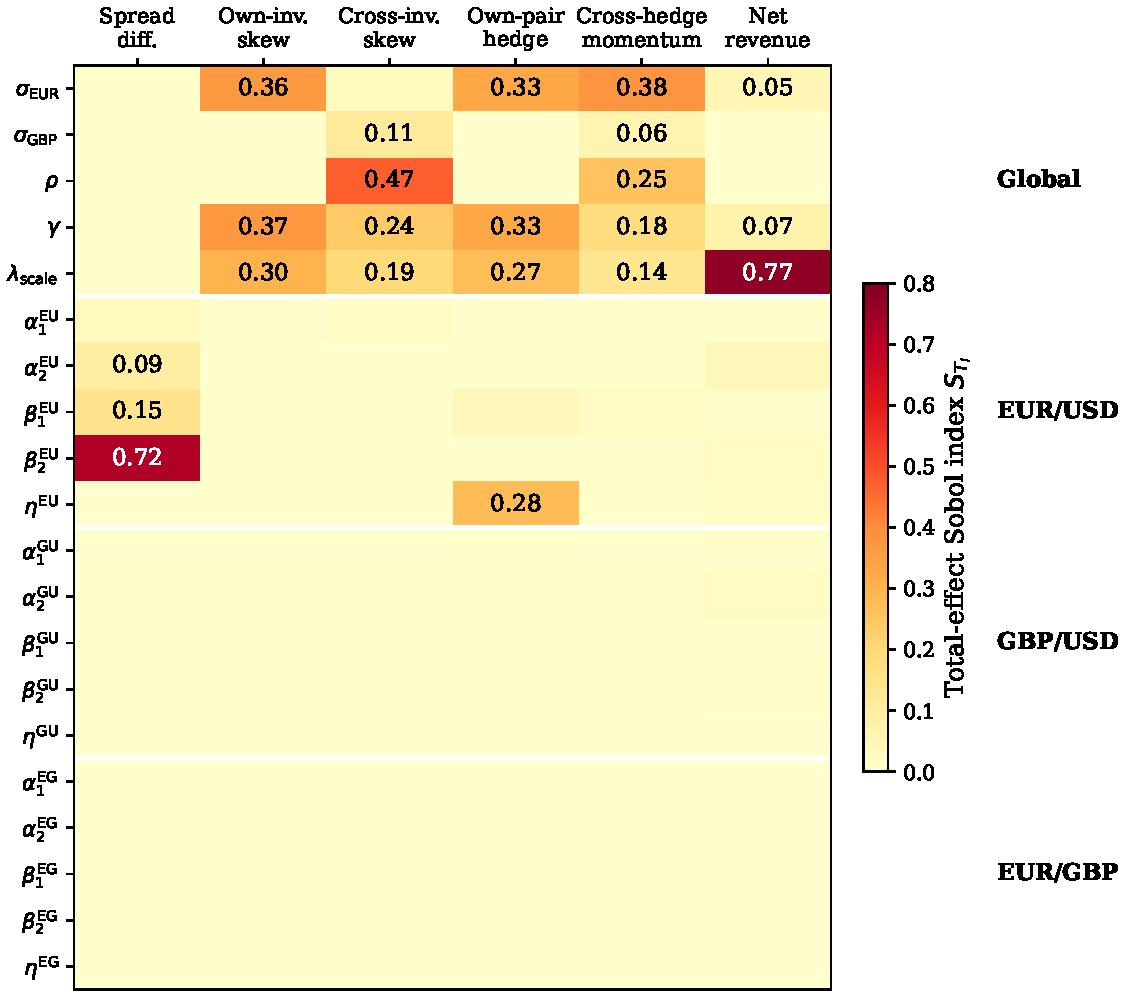
\includegraphics[width=0.75\textwidth]{figures/fig_sa_heatmap.pdf}
  \caption{Total-effect Sobol indices $S_{T_i}$ for 20 parameters (rows) and 6 quantities of interest (columns). Values above 0.05 are annotated. Parameters are grouped into global, EUR/USD, GBP/USD, and EUR/GBP. The block structure shows that different QoIs are sensitive to different parameter groups.}
  \label{fig:sa-heatmap}
\end{figure}


% ------------------------------------------------------------------
\subsection{Tier spread differential}
\label{sec:sa-qoi1}

The tier spread differential measures how much wider the model quotes for passive clients (tier~2) compared to aggressive clients (tier~1) on EURUSD at flat inventory. Figure~\ref{fig:sa-qoi1} shows the Sobol indices and output distribution.

\begin{figure}[ht]
  \centering
  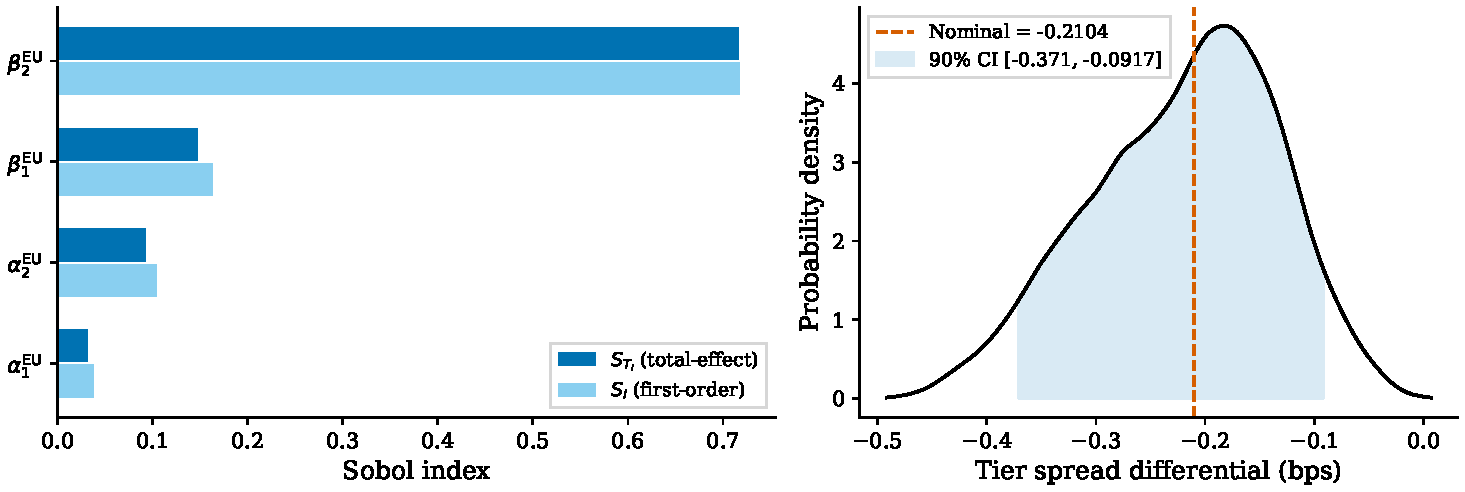
\includegraphics[width=\textwidth]{figures/fig_sa_qoi1.pdf}
  \caption{QoI~1: tier spread differential. Left: Sobol indices for parameters with $S_{T_i} > 0.02$. Right: output distribution from forward UQ ($n = 20{,}000$ samples), with nominal value (dashed red) and 90\% credible interval (shaded).}
  \label{fig:sa-qoi1}
\end{figure}

The tier spread differential is controlled entirely by the EUR/USD demand curve parameters. The passive-tier logistic slope $\beta_2^{\text{EU}}$ dominates ($S_i = 0.72$, $S_{T_i} = 0.72$), followed by $\beta_1^{\text{EU}}$ ($S_i = 0.17$, $S_{T_i} = 0.15$), $\alpha_2^{\text{EU}}$ ($S_i = 0.11$, $S_{T_i} = 0.09$), and $\alpha_1^{\text{EU}}$ ($S_i = 0.04$, $S_{T_i} = 0.03$). All other parameters, including all global parameters and all GBP/USD and EUR/GBP parameters, have $S_{T_i} < 0.001$. The first-order indices sum to 1.03 and the total-effect indices to 0.99; both estimates bracket 1 within Monte Carlo noise at $N = 10{,}000$, consistent with a perfectly additive model.

This result follows from the structure of the quoting formula. At zero inventory with $B(0) = 0$ (which holds under the direction-symmetric parameters of~\cite{barzykin2023}), the quoting momentum~\eqref{eq:p-formula} reduces to $p = z\,d^\T A(0)\,d$, which is small for the trade size $z = 1$\,M\$ considered here. The optimal markup is therefore dominated by the maximization of $f^n(\delta) \cdot \delta$ over the logistic demand curve, which depends only on the $(\alpha_n, \beta_n)$ of the two tiers being compared. The Riccati matrix $A(0)$ does depend on $\sigma$, $\gamma$, $\rho$, and $\lambda$ through the full dynamics~\eqref{eq:riccati-A}, but its contribution to the momentum~$p$ is negligible at this trade size.

A bank seeking to control its tiered client pricing therefore needs only to estimate the demand curves accurately. Volatility, risk aversion, and all cross-pair parameters are irrelevant for the flat-inventory spread differential. The forward UQ confirms moderate uncertainty (mean $= -0.22$\,bps, CV $= 39\%$, 90\% CI $= [-0.37, -0.09]$\,bps), reflecting the estimation error in the demand curve parameters.


% ------------------------------------------------------------------
\subsection{Own-inventory skew}
\label{sec:sa-qoi2}

The own-inventory skew measures how the EURUSD markup adjusts when the dealer holds 10\,M\$ in EUR. Figure~\ref{fig:sa-qoi2} shows the results.

\begin{figure}[ht]
  \centering
  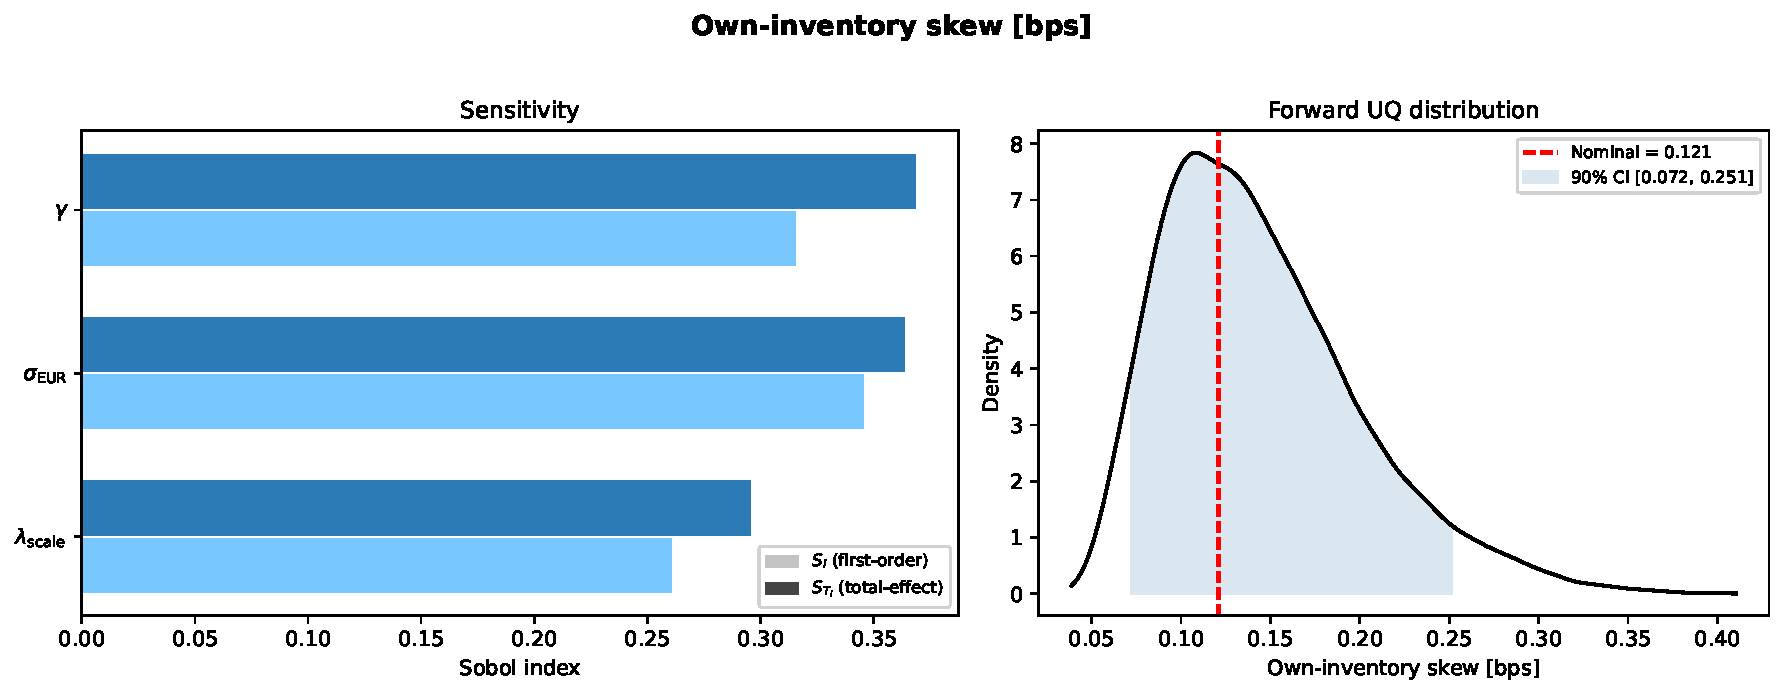
\includegraphics[width=\textwidth]{figures/fig_sa_qoi2.pdf}
  \caption{QoI~2: own-inventory skew. Left: Sobol indices. Right: output distribution.}
  \label{fig:sa-qoi2}
\end{figure}

The inventory skew is driven by three global parameters with roughly equal importance: $\sigma_{\text{EUR}}$ ($S_i = 0.35$, $S_{T_i} = 0.36$), $\gamma$ ($S_i = 0.32$, $S_{T_i} = 0.37$), and $\lambda_{\text{scale}}$ ($S_i = 0.26$, $S_{T_i} = 0.30$). All pair-specific parameters and the cross-pair parameters ($\sigma_{\text{GBP}}$, $\rho$) have $S_{T_i} < 0.01$. The model is nearly additive ($\sum S_i = 0.94$, $\sum S_{T_i} = 1.05$).

The skew arises from the value function gradient $2A(0)\,y$, and each of the three dominant parameters shapes the Riccati solution~$A$ through a different channel. Higher volatility increases inventory risk through the driving term $-\tfrac{\gamma}{2}\Sigma$ in~\eqref{eq:riccati-A}, enlarging~$A$ and hence the skew. Higher risk aversion amplifies this driving term directly. Higher arrival rates change the structure of the quoting Hamiltonian coefficients that enter the nonlinear term $2AMA$ in~\eqref{eq:riccati-A}, altering how the model balances quoting revenue against inventory risk. The demand curve parameters $(\alpha_n, \beta_n)$ affect the level of the spread but not its inventory dependence, because they enter through the Hamiltonian Taylor coefficients which scale~$A$ approximately uniformly.

The cross-pair parameters $\rho$ and $\sigma_{\text{GBP}}$ do not appear, even though they affect the diagonal entry $A_{\text{EUR,EUR}}$ through the Riccati coupling. The coupling's effect on the own-pair diagonal entries of~$A$ is too small to register at this sample size. The inventory adjustment of a single pair depends on the market environment (volatility, overall flow, risk preference) and is insensitive to the client demand model.

Forward UQ: mean $= 0.15$\,bps, CV $= 38\%$, 90\% CI $= [0.07, 0.25]$\,bps. The nominal value of 0.12\,bps falls below the mean because the uniform range for~$\gamma$ ($[10, 40]$, midpoint 25) lies above the nominal value of 20, pulling the average skew upward.


% ------------------------------------------------------------------
\subsection{Cross-inventory skew}
\label{sec:sa-qoi3}

The cross-inventory skew measures how GBP inventory shifts the EURUSD markup, probing the cross-currency coupling through the off-diagonal entries of~$A$. Figure~\ref{fig:sa-qoi3} shows the results.

\begin{figure}[ht]
  \centering
  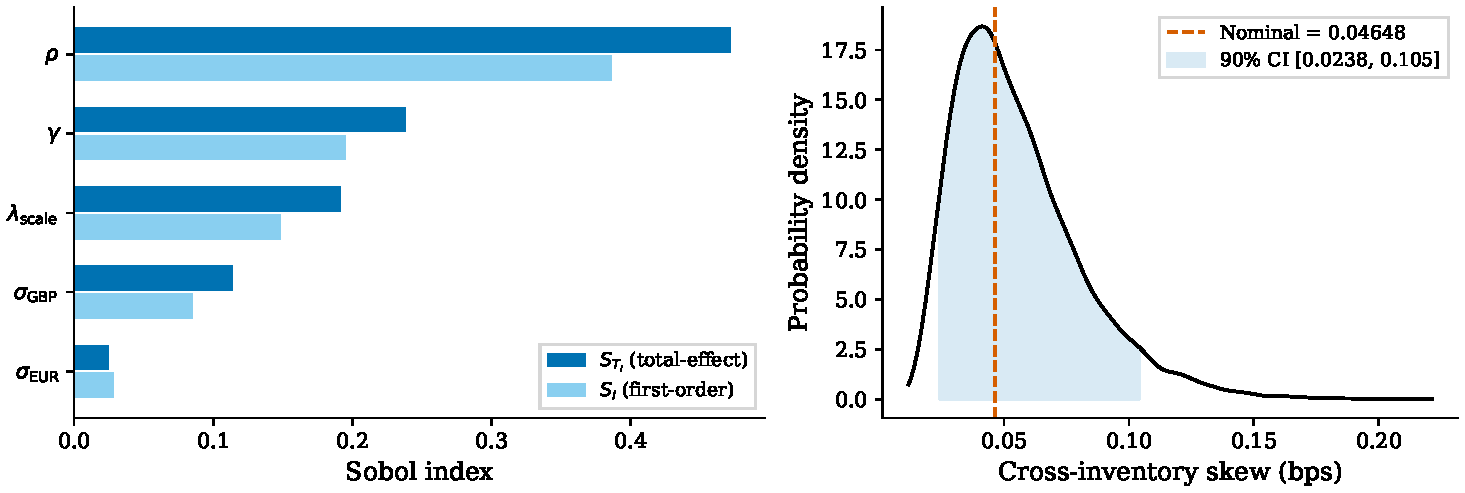
\includegraphics[width=\textwidth]{figures/fig_sa_qoi3.pdf}
  \caption{QoI~3: cross-inventory skew. Left: Sobol indices. Right: output distribution. The 90\% CI is entirely positive, confirming that the cross-pair coupling is a structural feature, not noise.}
  \label{fig:sa-qoi3}
\end{figure}

The cross-inventory skew is primarily driven by the correlation $\rho$ ($S_i = 0.39$, $S_{T_i} = 0.47$), confirming that correlation is the gateway to all cross-pair effects. The risk aversion~$\gamma$ ($S_i = 0.20$, $S_{T_i} = 0.24$) and arrival rate scale $\lambda_{\text{scale}}$ ($S_i = 0.15$, $S_{T_i} = 0.19$) are secondary drivers. The GBP volatility $\sigma_{\text{GBP}}$ appears at a lower level ($S_i = 0.09$, $S_{T_i} = 0.12$), and EUR volatility $\sigma_{\text{EUR}}$ registers a minor contribution. The gap between $S_i$ and $S_{T_i}$ for $\rho$ (0.39 vs.\ 0.47) indicates moderate interaction with the other global parameters. The total-effect indices sum to 1.08, so the model is nearly additive with a modest interaction contribution concentrated on~$\rho$.

The cross-inventory skew depends on the off-diagonal entries of~$A$ that couple GBP to the EUR/USD quoting momentum. These entries arise from the correlation entering the Riccati driving term $-\tfrac{\gamma}{2}\Sigma$: the off-diagonal covariance is $\Sigma_{\text{EUR,GBP}} = \rho\,\sigma_{\text{EUR}}\,\sigma_{\text{GBP}}$, so when $\rho = 0$ the off-diagonal of~$\Sigma$ vanishes, $A_{\text{EUR,GBP}} = 0$, and the cross-skew is zero. The GBP volatility $\sigma_{\text{GBP}}$ enters for the same reason: it scales the off-diagonal covariance that generates the cross-pair coupling.

One might expect that demand parameters of one pair could affect the strategy for another pair, since the Riccati matrices $M$, $\tilde{M}$, and $P$ aggregate Hamiltonian coefficients from all three pairs. The Sobol analysis shows that this coupling is negligible: no cross-pair demand parameter has $S_{T_i} > 0.015$ for the cross-inventory skew. Cross-pair effects propagate through the covariance matrix, not through client flow characteristics.

The forward UQ shows a mean cross-skew of 0.055\,bps with CV $= 46\%$ and a 90\% CI of $[0.024, 0.105]$\,bps. The CI is entirely positive: the cross-pair coupling is consistently nonzero across the parameter space. The magnitude is about 38\% of the own-inventory skew (mean 0.15\,bps), confirming that cross-pair coupling is a genuine structural feature of the multi-currency model, large enough to be practically relevant for a bank managing multiple currency desks.


% ==================================================================
\section{Results: hedging and economics (Set B)}
\label{sec:sa-results-b}


% ------------------------------------------------------------------
\subsection{Own-pair hedge rate}
\label{sec:sa-qoi4}

The own-pair hedge rate measures how aggressively the model hedges EUR exposure through the EURUSD interbank market. Figure~\ref{fig:sa-qoi4} shows the results.

\begin{figure}[ht]
  \centering
  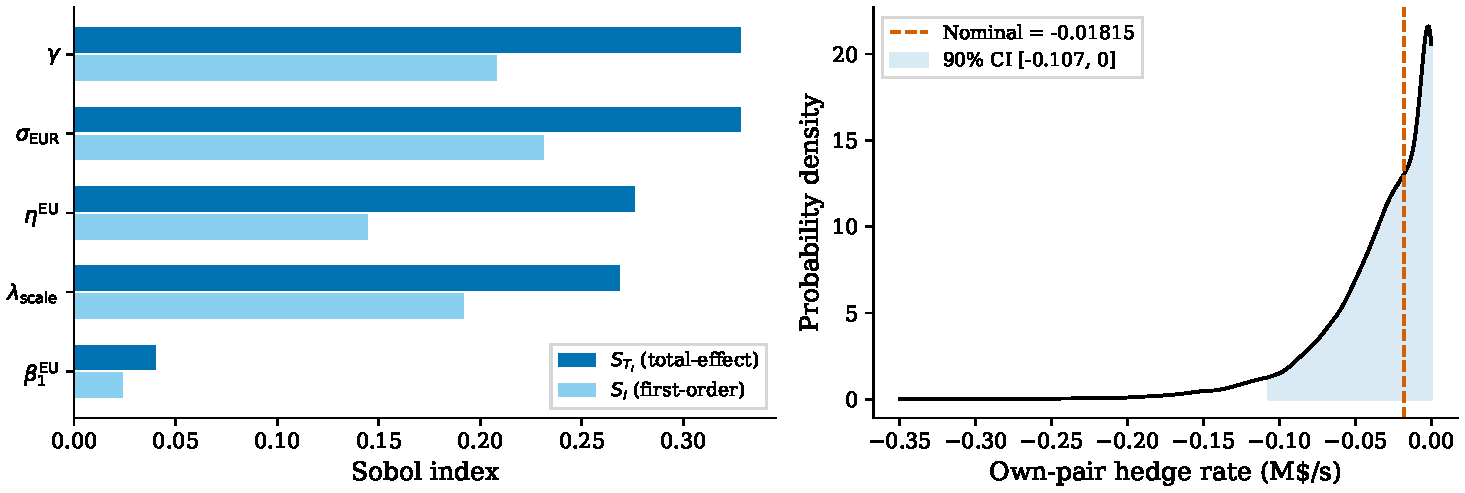
\includegraphics[width=\textwidth]{figures/fig_sa_qoi4.pdf}
  \caption{QoI~4: own-pair hedge rate. Left: Sobol indices, showing the largest gap between $S_i$ and $S_{T_i}$ for~$\eta^{\text{EU}}$ (strong interactions). Right: output distribution, with CV $= 111\%$.}
  \label{fig:sa-qoi4}
\end{figure}

Four parameters contribute: $\sigma_{\text{EUR}}$ ($S_i = 0.23$, $S_{T_i} = 0.33$), $\gamma$ ($S_i = 0.21$, $S_{T_i} = 0.33$), $\lambda_{\text{scale}}$ ($S_i = 0.19$, $S_{T_i} = 0.27$), and $\eta^{\text{EU}}$ ($S_i = 0.15$, $S_{T_i} = 0.28$). No cross-pair parameter has $S_{T_i} > 0.01$. The total-effect indices sum to 1.26, the highest of any QoI, indicating significant interaction effects.

The interactions arise from the hedge rate formula. Outside the dead zone, $\xi^* = (p - \psi)/(2\eta)$, where the hedging momentum~$p$ depends on the value function gradient and hence on $\sigma$, $\gamma$, and~$\lambda$ through the Riccati solution. The execution cost~$\eta$ enters multiplicatively with~$p$: changing~$\eta$ amplifies or dampens the effect of every parameter that influences the gradient. This multiplicative coupling explains why $\eta^{\text{EU}}$ has the largest gap between $S_i$ and $S_{T_i}$ ($0.15$ vs.\ $0.28$, a ratio of nearly 2).

The cross-pair parameters do not affect own-pair hedging. Although the model has EURGBP available as an alternative hedge instrument, the EURGBP dead zone blocks cross-hedging for nearly all parameter combinations (see QoI~5 below), so the EURUSD hedge rate is determined as if it were the only hedging channel.

The forward UQ confirms that the hedge rate is the least robust component of the strategy: mean $= -0.0335$\,M\$/s, standard deviation $= 0.0372$, CV $= 111\%$, 90\% CI $= [-0.107,\; 0]$\,M\$/s. The CI spans more than an order of magnitude. The distribution is heavily left-skewed because small values of~$\eta$ produce extremely large hedge rates through the $1/(2\eta)$ factor. The upper end of the CI reaches zero, meaning that for some parameter combinations the hedging momentum falls within the dead zone and the model prescribes no hedging at all.


% ------------------------------------------------------------------
\subsection{Cross-hedge momentum}
\label{sec:sa-qoi5}

Chapter~\ref{ch:ode} showed that the model hedges EUR exposure through multiple pairs, including the cross pair EURGBP (Figure~\ref{fig:ode-hedging}). To measure the sensitivity of this cross-hedging channel, we examine the value function's incentive to cross-hedge: the raw hedging momentum~$p_{\text{EURGBP}}$ before the dead zone clips it. Figure~\ref{fig:sa-qoi5} shows the results.

\begin{figure}[ht]
  \centering
  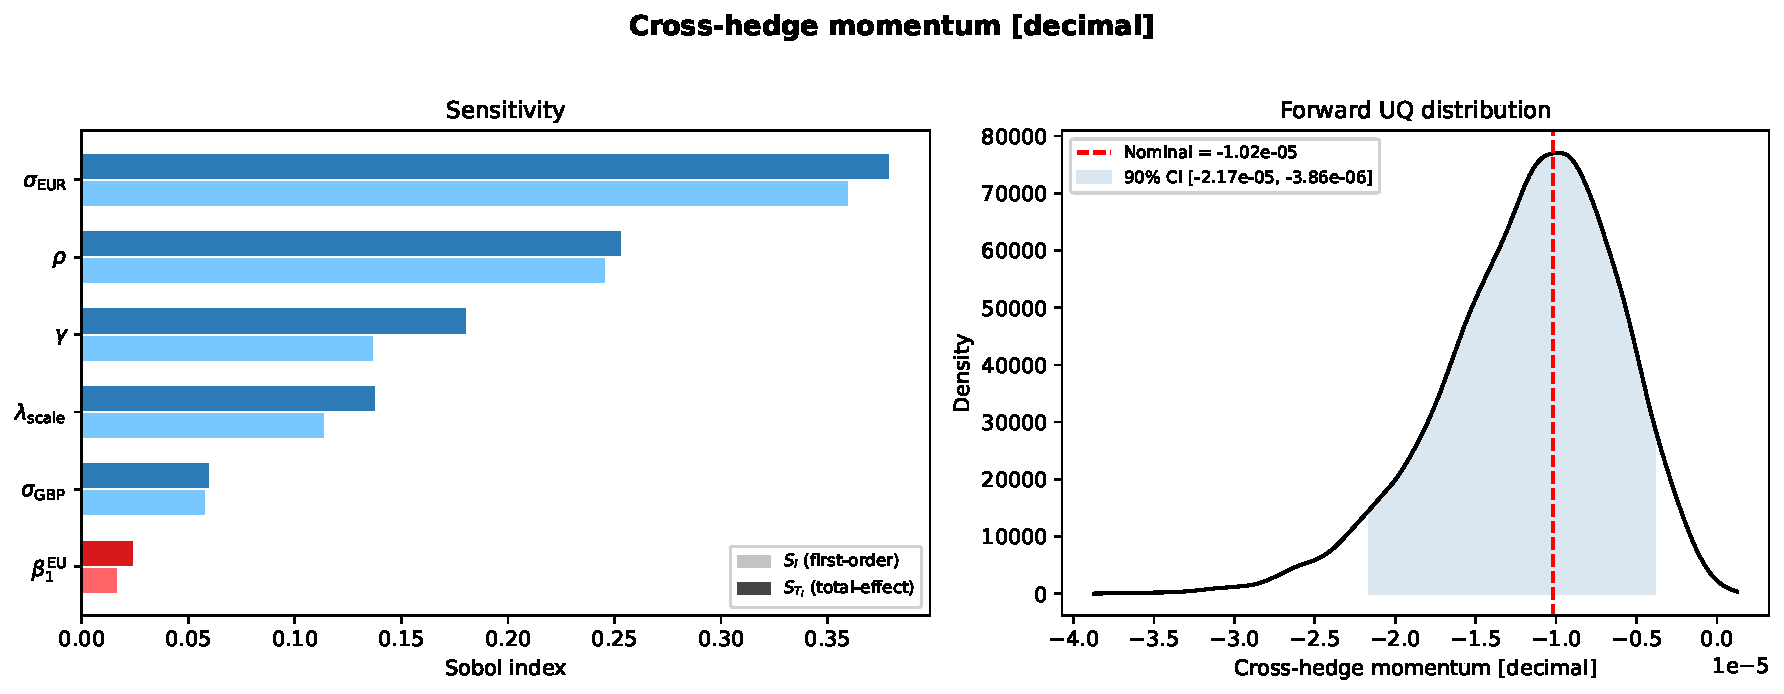
\includegraphics[width=\textwidth]{figures/fig_sa_qoi5.pdf}
  \caption{QoI~5: cross-hedge momentum. Left: Sobol indices. Right: output distribution. The momentum is consistently negative (the model wants to sell EUR / buy GBP to hedge), but its magnitude is smaller than the EURGBP dead zone.}
  \label{fig:sa-qoi5}
\end{figure}

The cross-hedge momentum is driven entirely by global parameters: $\sigma_{\text{EUR}}$ ($S_i = 0.36$, $S_{T_i} = 0.38$), $\rho$ ($S_i = 0.25$, $S_{T_i} = 0.25$), $\gamma$ ($S_i = 0.14$, $S_{T_i} = 0.18$), $\lambda_{\text{scale}}$ ($S_i = 0.11$, $S_{T_i} = 0.14$), and $\sigma_{\text{GBP}}$ ($S_i = 0.06$, $S_{T_i} = 0.06$). The model is nearly additive ($\sum S_{T_i} = 1.05$). No pair-specific execution cost appears and no demand parameter has $S_{T_i} > 0.03$, because the momentum measures the value function gradient directly, before any clipping or scaling by~$\eta$.

EUR volatility dominates rather than $\rho$ because the momentum depends on $A_{\text{EUR,EUR}} - A_{\text{GBP,EUR}}$. The diagonal entry $A_{\text{EUR,EUR}}$ scales strongly with $\sigma_{\text{EUR}}$ through the Riccati driving term $-\tfrac{\gamma}{2}\Sigma$, while $\rho$ controls only the off-diagonal entry $A_{\text{GBP,EUR}}$. The diagonal contribution is larger in magnitude, giving $\sigma_{\text{EUR}}$ a higher Sobol index.

The forward UQ shows a mean momentum of $-1.17 \times 10^{-5}$ (decimal) with CV $= 46\%$ and 90\% CI $= [-2.17, -0.39] \times 10^{-5}$. The momentum is consistently negative: the value function pushes toward selling EUR and buying GBP to reduce correlated risk. However, the EURGBP dead zone is $\psi_{\text{EG}} = 2.5 \times 10^{-5}$ in decimal units, which exceeds the typical momentum magnitude. Cross-hedging is structurally present in the value function but economically blocked by execution costs at the paper's parameter values. A more liquid cross pair (lower~$\psi$, lower~$\eta$) could unlock this channel.


% ------------------------------------------------------------------
\subsection{Net revenue}
\label{sec:sa-qoi6}

The net revenue aggregates quoting revenue across all three pairs minus total hedging cost, evaluated at the long-EUR inventory state. Figure~\ref{fig:sa-qoi6} shows the results.

\begin{figure}[ht]
  \centering
  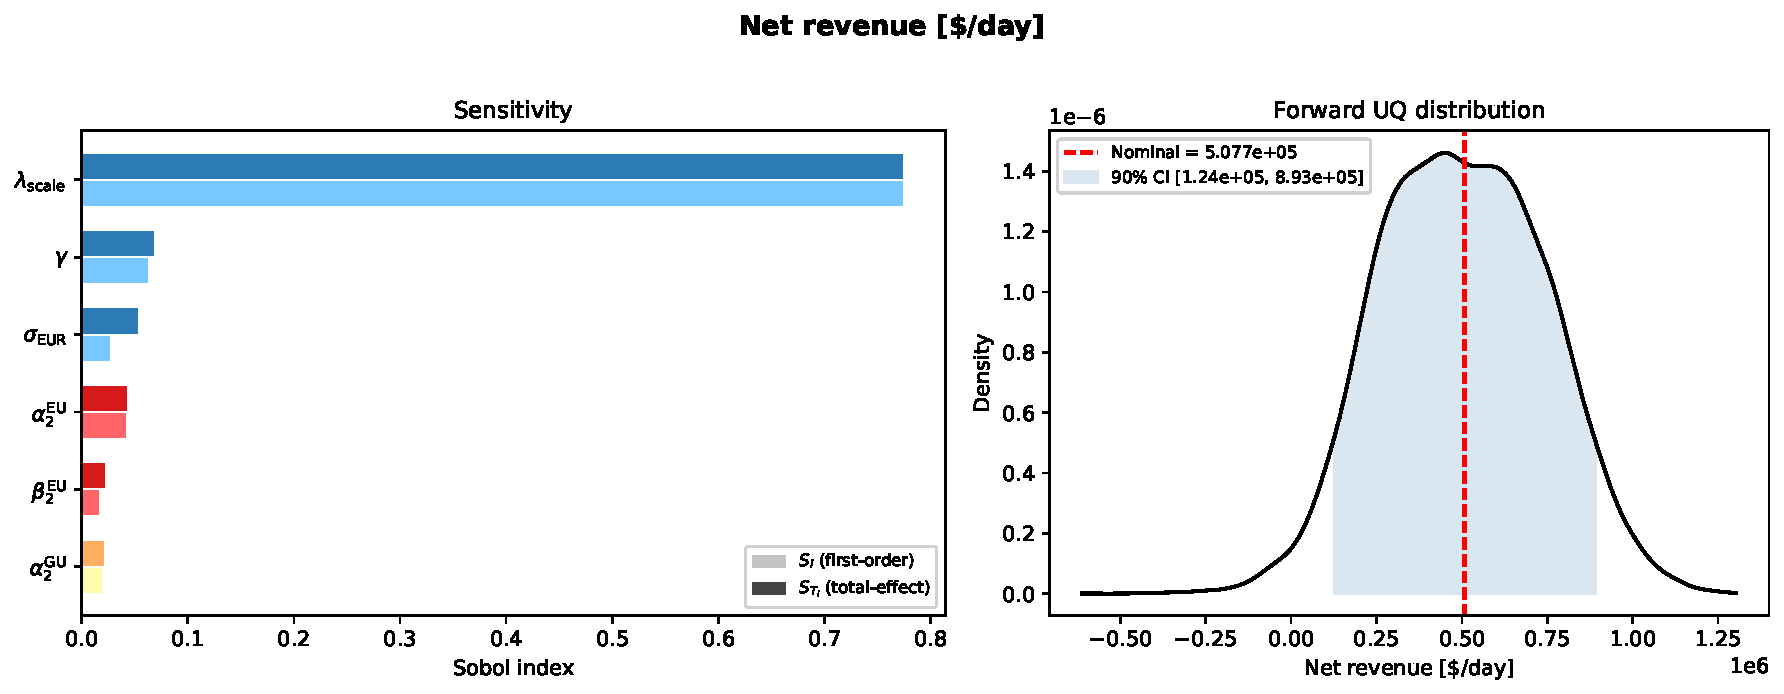
\includegraphics[width=\textwidth]{figures/fig_sa_qoi6.pdf}
  \caption{QoI~6: net revenue. Left: Sobol indices, dominated by $\lambda_{\text{scale}}$ ($S_{T_i} = 0.78$). Right: output distribution, with 90\% CI entirely positive.}
  \label{fig:sa-qoi6}
\end{figure}

The arrival rate scale $\lambda_{\text{scale}}$ dominates ($S_i = 0.78$, $S_{T_i} = 0.78$). Revenue is roughly proportional to total client flow, and $\lambda_{\text{scale}}$ scales all arrival rates across all three pairs. The model is nearly additive ($\sum S_i = 0.99$, $\sum S_{T_i} = 1.05$). Secondary contributors are $\gamma$ ($S_i = 0.06$, $S_{T_i} = 0.07$), $\alpha_2^{\text{EU}}$ ($S_i = 0.04$, $S_{T_i} = 0.04$), and $\sigma_{\text{EUR}}$ ($S_i = 0.03$, $S_{T_i} = 0.05$), along with $\alpha_2^{\text{GU}}$ and $\beta_2^{\text{EU}}$ at $S_{T_i} \approx 0.02$. This is the only QoI where GBP/USD demand parameters appear with nonzero Sobol indices, because net revenue sums contributions from all three pairs.

The forward UQ gives
\[
  \text{mean} = \$502\text{k/day}, \qquad \text{CV} = 48\%, \qquad 90\%\ \text{CI} = [\$124\text{k},\; \$893\text{k}]/\text{day}.
\]
The CI is entirely positive: the strategy is profitable across every parameter combination in the sample. The main source of revenue uncertainty is simply how much client flow the desk receives, not the risk management parameters.


% ==================================================================
\section{Discussion}
\label{sec:sa-discussion}

% ------------------------------------------------------------------
\subsection{Sensitivity structure}
\label{sec:sa-sensitivity-structure}

The central finding of the analysis is that different aspects of the market making strategy are sensitive to entirely different parameters. Table~\ref{tab:sa-summary} summarizes the dominant parameters and the degree of interaction for each QoI.

\begin{table}[ht]
\centering
\caption{Summary of the sensitivity structure. For each QoI, the dominant parameters (those with $S_{T_i} > 0.05$) and the presence of interactions ($\sum S_{T_i}$ relative to~1) are listed.}
\label{tab:sa-summary}
\begin{tabular}{@{}llc@{}}
\toprule
Quantity of interest & Dominant parameters & Interactions \\
\midrule
Tier spread differential (QoI~1) & $\beta_2^{\text{EU}}$, $\beta_1^{\text{EU}}$, $\alpha_2^{\text{EU}}$ & None \\
Own-inventory skew (QoI~2) & $\sigma_{\text{EUR}}$, $\gamma$, $\lambda_{\text{scale}}$ & Small \\
Cross-inventory skew (QoI~3) & $\rho$, $\gamma$, $\lambda_{\text{scale}}$, $\sigma_{\text{GBP}}$ & Small \\
Own-pair hedge rate (QoI~4) & $\sigma_{\text{EUR}}$, $\gamma$, $\lambda_{\text{scale}}$, $\eta^{\text{EU}}$ & Significant \\
Cross-hedge momentum (QoI~5) & $\sigma_{\text{EUR}}$, $\rho$, $\gamma$, $\lambda_{\text{scale}}$, $\sigma_{\text{GBP}}$ & Small \\
Net revenue (QoI~6) & $\lambda_{\text{scale}}$, $\gamma$, $\sigma_{\text{EUR}}$ & Small \\
\bottomrule
\end{tabular}
\end{table}

The separation falls along clear lines. The tier spread differential is a \emph{microstructure} quantity: it depends only on the shape of the client demand curves and is insensitive to market-level conditions. The inventory skew and hedge rate are \emph{risk management} quantities: they depend on volatility, risk preference, and market activity, with the hedge rate additionally sensitive to execution cost. The cross-pair quantities (QoIs~3 and~5) introduce the correlation~$\rho$ as a new dimension that does not appear for any own-pair quantity. Net revenue is dominated by a single parameter, the overall level of client flow.


% ------------------------------------------------------------------
\subsection{Robustness of the optimal strategy}
\label{sec:sa-robustness}

The forward uncertainty quantification reveals a gradient of robustness across the strategy's components. Table~\ref{tab:sa-forward-uq} summarizes the output distributions.

\begin{table}[ht]
\centering
\caption{Forward uncertainty quantification results. The coefficient of variation (CV) measures the relative spread of each output distribution. Sample size $2N = 20{,}000$.}
\label{tab:sa-forward-uq}
\begin{tabular}{@{}lcccc@{}}
\toprule
QoI & Mean & Std & 90\% CI & CV \\
\midrule
Tier spread diff.\ [bps]       & $-0.22$ & 0.09 & $[-0.37,\; -0.09]$ & 39\% \\
Own-inv.\ skew [bps]           & $0.15$ & 0.06 & $[0.07,\; 0.25]$ & 38\% \\
Cross-inv.\ skew [bps]         & $0.055$ & 0.026 & $[0.024,\; 0.105]$ & 46\% \\
Own-pair hedge [M\$/s]         & $-0.0335$ & 0.0372 & $[-0.107,\; 0]$ & 111\% \\
Cross-hedge mom.\ [decimal]    & $-1.17 \times 10^{-5}$ & $5.4 \times 10^{-6}$ & $[-2.2,\; -0.4] \times 10^{-5}$ & 46\% \\
Net revenue [\$/day]           & $502{,}000$ & 240{,}000 & $[124\text{k},\; 893\text{k}]$ & 48\% \\
\bottomrule
\end{tabular}
\end{table}

The quoting policy is relatively robust, with CVs of 38--46\% for the spread differential, own-inventory skew, and cross-inventory skew. These outputs are stable under parameter uncertainty: the spreads and inventory adjustments change, but not by an order of magnitude. The hedge rate is a different story. With a CV of 111\% and a 90\% CI spanning from $-0.108$ to 0\,M\$/s, the model's hedging prescription is highly uncertain. The distribution is heavily left-skewed because small values of~$\eta$ produce extremely large hedge rates through the $1/(2\eta)$ factor.

Figure~\ref{fig:sa-scatter-eta} makes this nonlinearity visible. The scatter plot of $\eta^{\text{EU}}$ versus the own-pair hedge rate shows the hyperbolic $1/\eta$ relationship: as $\eta$ decreases from $2 \times 10^{-5}$ to $0.5 \times 10^{-5}$, the hedge rate magnitude explodes from around $-0.012$ to beyond $-0.12$\,M\$/s. Underestimating market impact by a factor of two can lead to a factor-of-two overestimate of the optimal hedging rate.

\begin{figure}[ht]
  \centering
  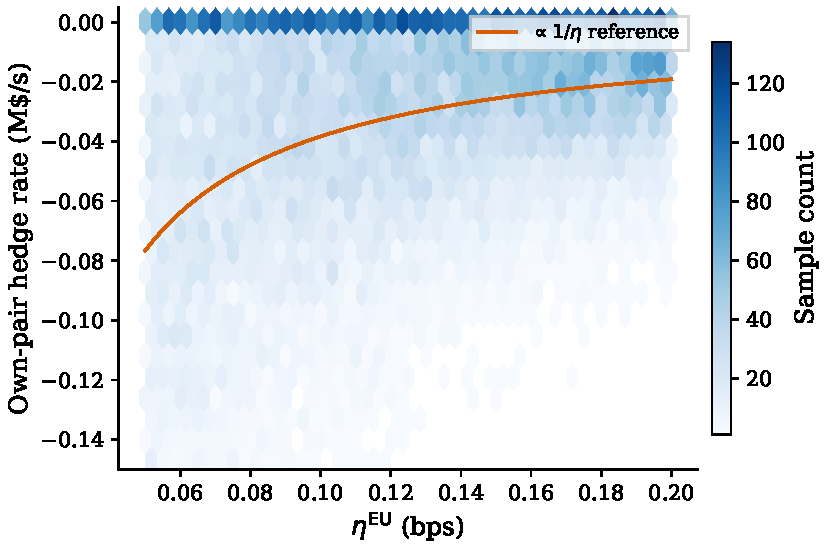
\includegraphics[width=0.6\textwidth]{figures/fig_sa_scatter_eta_hedge.pdf}
  \caption{Scatter plot of $\eta^{\text{EU}}$ versus the own-pair hedge rate ($n = 20{,}000$ samples). The red curve shows the $1/\eta$ reference scaling. The enormous spread at low~$\eta$ values reflects the multiplicative interaction with other parameters.}
  \label{fig:sa-scatter-eta}
\end{figure}

Figure~\ref{fig:sa-scatter-rho} illustrates a different type of sensitivity: the approximately linear relationship between~$\rho$ and the cross-inventory skew. As the correlation increases from 0.3 to 0.9, the cross-skew roughly doubles. This is consistent with the mechanism identified in Section~\ref{sec:sa-qoi3}: correlation controls the off-diagonal covariance $\Sigma_{\text{EUR,GBP}} = \rho\,\sigma_{\text{EUR}}\,\sigma_{\text{GBP}}$, which is the primary source of the cross-pair coupling in the Riccati equation. The vertical spread at each $\rho$ value reflects the combined effect of the other global parameters ($\gamma$, $\lambda_{\text{scale}}$, $\sigma_{\text{GBP}}$).

\begin{figure}[ht]
  \centering
  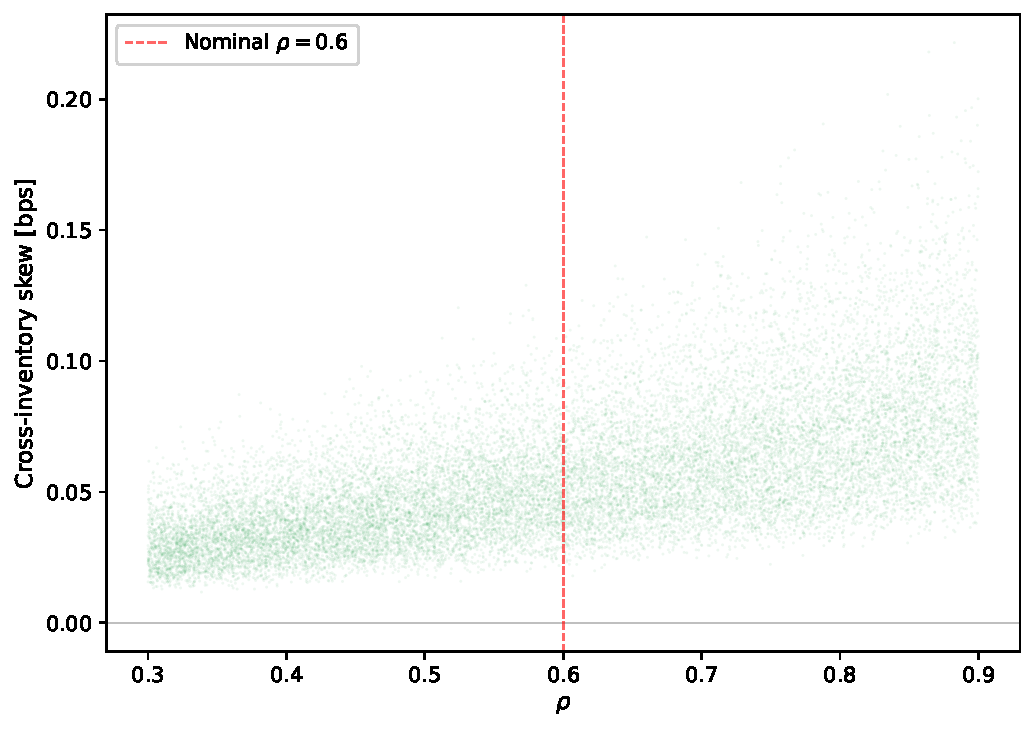
\includegraphics[width=0.6\textwidth]{figures/fig_sa_scatter_rho_cross.pdf}
  \caption{Correlation~$\rho$ versus cross-inventory skew ($n = 20{,}000$ samples). The linear fit confirms the approximately linear relationship: the cross-skew roughly doubles from low to high correlation.}
  \label{fig:sa-scatter-rho}
\end{figure}

The net revenue remains positive across the entire parameter space explored (90\% CI $= [\$124\text{k},\; \$893\text{k}]$/day). The strategy is profitable regardless of the parameter combination. The main risk under parameter uncertainty is not that the strategy loses money, but that the hedging prescriptions may be unreliable: the desk does not know how aggressively to hedge, even though it knows it will be profitable.


% ------------------------------------------------------------------
\subsection{Practical implications}
\label{sec:sa-practical}

The sensitivity analysis has concrete consequences for a desk deploying this model. The quoting policy is the most reliable component: with CVs of 38--46\%, the tier spreads and inventory skew the model produces are stable under parameter uncertainty. A desk can set its client-facing quotes from the model with reasonable confidence, even if the underlying parameters carry estimation error.

The hedging prescription is less reliable. With a CV of 111\%, the model's hedge rate is highly sensitive to the market impact parameter~$\eta$: the $1/(2\eta)$ factor means that small errors in the~$\eta$ estimate produce large swings in the prescribed hedging speed. The model identifies \emph{whether} to hedge and in \emph{which direction}, but the aggressiveness of hedging should be treated as a guide rather than a hard prescription. Real-time monitoring or trader oversight on hedging speed is warranted.

Calibration effort should be targeted accordingly. Each pair's quoting depends on its own demand curve parameters ($\alpha_n$, $\beta_n$), while the risk management quantities depend on the global parameters ($\sigma$, $\rho$, $\gamma$, $\lambda_{\text{scale}}$) and the own-pair execution cost~$\eta$. Cross-pair demand parameters have negligible effect. These two groups also evolve differently: the global parameters reflect market conditions that shift daily and benefit from frequent recalibration, while the demand curves describe client behavior and change more slowly. In particular, a desk should monitor the correlation~$\rho$ closely, as the cross-inventory effect on quoting roughly doubles between low and high correlation regimes (Figure~\ref{fig:sa-scatter-rho}), making cross-pair positions more relevant for quoting during correlated markets.

Despite the hedge rate uncertainty, the strategy's profitability is not in question. The net revenue 90\% CI is entirely positive (Table~\ref{tab:sa-forward-uq}). The risk under parameter uncertainty is not that the desk loses money, but that it hedges too aggressively or too passively, affecting the efficiency of the strategy rather than its sign.


% ------------------------------------------------------------------
\subsection{Connection to the PDE solution}
\label{sec:sa-bridge}

All results in this chapter are based on the ODE approximation, which replaces the exact Hamiltonians with quadratic Taylor expansions around zero quoting momentum. In Chapter~\ref{ch:pde}, we develop a grid-based PDE solver for the full HJB equation in the two-currency case and compare the ODE and PDE solutions across a range of parameter regimes. This comparison verifies whether the sensitivity conclusions derived here carry over to the exact solution, or whether the quadratic approximation introduces biases that alter the sensitivity structure.
